\section{Familias de Optimizadores y Dinámicas de Entrenamiento}
\label{sec:optimizer-families}

Optimizar arquitecturas transformer grandes se complica por paisajes no convexos, puntos de silla y grupos de parámetros heterogéneos. El sistema soporta veinticuatro familias de optimizadores en siete categorías: líneas base clásicas (SGD con momentum, AdamW, RAdam); momentum y reducción de varianza (Adan, ADOPT, AdEMAMix, MARS, Cautious AdamW); métodos eficientes en memoria y de bajo rango (Adafactor, GaLore, Lion, APOLLO, APOLLO-Mini, Q-APOLLO); métodos sin programación y sin parámetros (Schedule-Free AdamW, Prodigy) con escalado para lotes grandes (LAMB); métodos conscientes de la curvatura y de segundo orden (Sophia, Shampoo, SOAP); métodos orientados a geometría (Muon, Turbo-Muon, AF-Muon); y optimizadores de adaptividad ajustable (Anon). Los algoritmos, el pseudocódigo y las comparaciones de memoria y complejidad se recopilan en el Apéndice~\ref{sec:annex-optimizers}.

\begin{figure}[t]
\centering
\fitfigure{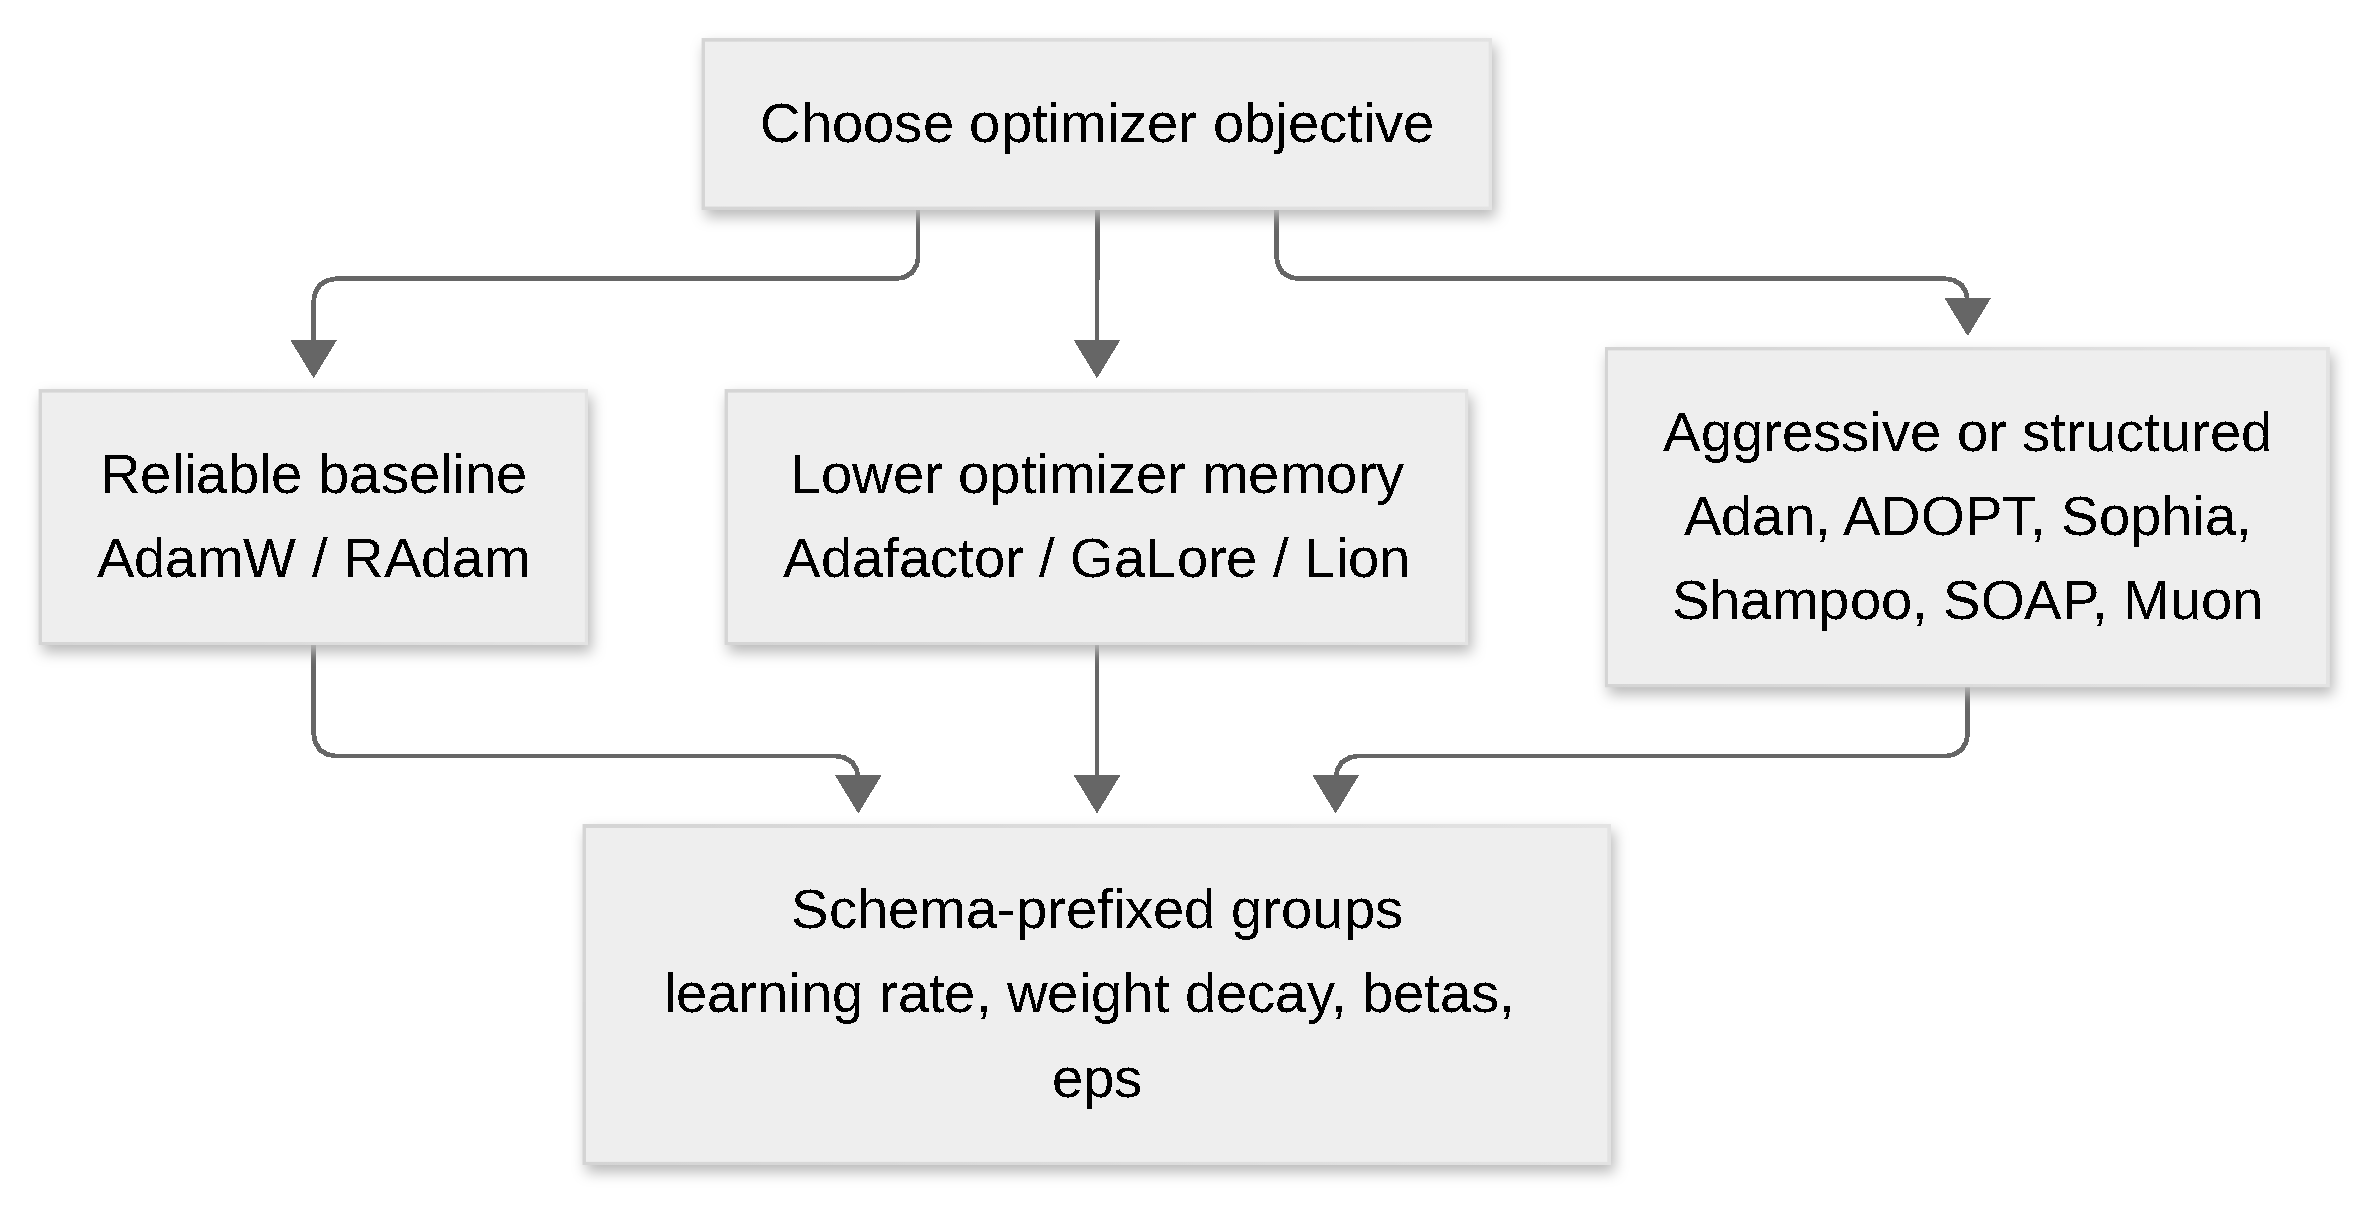
\includegraphics{../paper/figures/optimizer-routing.pdf}}
\caption{Selección de optimizador en la práctica: la clase determina la regla de actualización, mientras que el esquema controla cómo se aplican los hiperparámetros en los diez bloques canónicos de parámetros (embeddings, encodings posicionales, atención, feed-forward, normalización, heads, mHC, routers, residuales y el resto de parámetros).}
\label{fig:optimizer-routing}
\end{figure}
